\section{Risk and Technical Debt}

To measure the risks of this project we will use the following 3x3 risk matrix, which will help us develop the 
\gls{risk assessment}:

\begin{figure}[H]
    \centering
    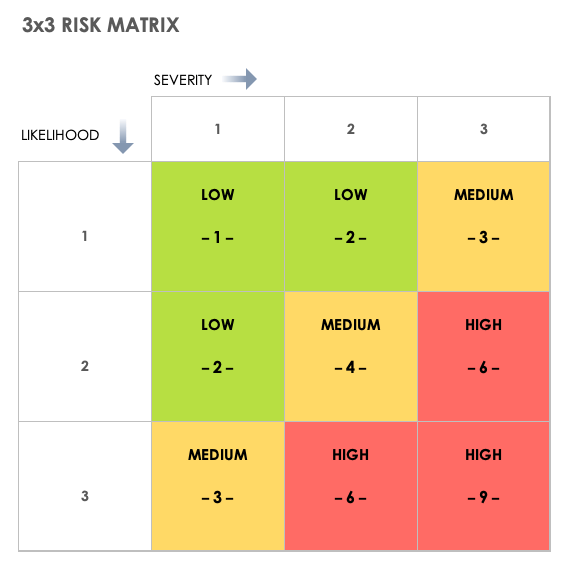
\includegraphics[width=0.5\textwidth]{assets/Risk-Matrix.png}
    \caption{3x3 Risk Matrix Template\\ Source: \citet{refonline:smtrisk}  }
    \label{fig:risk_matrix_template}
\end{figure}

The elements used to identify the risk are shown in the figure \ref{fig:technical_context}. The table below represents
the identified risk value:

\newpage
\thispagestyle{lscape}
\begin{landscape}

    \begin{table}[H]
        \setstretch{1.0}
        \begin{tabularx}{\textwidth}{|X|c|c|c|c|c|c|}
            \toprule
            \multicolumn{1}{c}{\textbf{Risk Criteria} } & \multicolumn{1}{X}{Client Graphical Interface} & \multicolumn{1}{X}{Provider Graphical Interface} &
            \multicolumn{1}{c}{Offer Database } & \multicolumn{1}{c}{API} & \multicolumn{1}{X}{External Payment Service}  &
            \multicolumn{1}{c}{External Login/Registration Service} \\
            \midrule
            Unproven technology         &  &  &  &  &  & \\
            \hline
            Performancey                &  &  &  &  &  & \\
            \hline
            Scalability                 &  &  &  &  &  & \\
            \hline
            Availability                &  &  &  &  &  & \\
            \hline
            Data loss                   &  &  &  &  &  & \\
            \hline
            Single points of failure    &  &  &  &  &  & \\
            \hline
            Security                    &  &  &  &  &  & \\
            \hline
            \bottomrule
        \end{tabularx}
    \end{table}

\end{landscape}






